% Options for packages loaded elsewhere
\PassOptionsToPackage{unicode}{hyperref}
\PassOptionsToPackage{hyphens}{url}
%
\documentclass[
]{article}
\usepackage{amsmath,amssymb}
\usepackage{iftex}
\ifPDFTeX
  \usepackage[T1]{fontenc}
  \usepackage[utf8]{inputenc}
  \usepackage{textcomp} % provide euro and other symbols
\else % if luatex or xetex
  \usepackage{unicode-math} % this also loads fontspec
  \defaultfontfeatures{Scale=MatchLowercase}
  \defaultfontfeatures[\rmfamily]{Ligatures=TeX,Scale=1}
\fi
\usepackage{lmodern}
\ifPDFTeX\else
  % xetex/luatex font selection
\fi
% Use upquote if available, for straight quotes in verbatim environments
\IfFileExists{upquote.sty}{\usepackage{upquote}}{}
\IfFileExists{microtype.sty}{% use microtype if available
  \usepackage[]{microtype}
  \UseMicrotypeSet[protrusion]{basicmath} % disable protrusion for tt fonts
}{}
\makeatletter
\@ifundefined{KOMAClassName}{% if non-KOMA class
  \IfFileExists{parskip.sty}{%
    \usepackage{parskip}
  }{% else
    \setlength{\parindent}{0pt}
    \setlength{\parskip}{6pt plus 2pt minus 1pt}}
}{% if KOMA class
  \KOMAoptions{parskip=half}}
\makeatother
\usepackage{xcolor}
\usepackage[margin=1in]{geometry}
\usepackage{graphicx}
\makeatletter
\def\maxwidth{\ifdim\Gin@nat@width>\linewidth\linewidth\else\Gin@nat@width\fi}
\def\maxheight{\ifdim\Gin@nat@height>\textheight\textheight\else\Gin@nat@height\fi}
\makeatother
% Scale images if necessary, so that they will not overflow the page
% margins by default, and it is still possible to overwrite the defaults
% using explicit options in \includegraphics[width, height, ...]{}
\setkeys{Gin}{width=\maxwidth,height=\maxheight,keepaspectratio}
% Set default figure placement to htbp
\makeatletter
\def\fps@figure{htbp}
\makeatother
\setlength{\emergencystretch}{3em} % prevent overfull lines
\providecommand{\tightlist}{%
  \setlength{\itemsep}{0pt}\setlength{\parskip}{0pt}}
\setcounter{secnumdepth}{-\maxdimen} % remove section numbering
% definitions for citeproc citations
\NewDocumentCommand\citeproctext{}{}
\NewDocumentCommand\citeproc{mm}{%
  \begingroup\def\citeproctext{#2}\cite{#1}\endgroup}
\makeatletter
 % allow citations to break across lines
 \let\@cite@ofmt\@firstofone
 % avoid brackets around text for \cite:
 \def\@biblabel#1{}
 \def\@cite#1#2{{#1\if@tempswa , #2\fi}}
\makeatother
\newlength{\cslhangindent}
\setlength{\cslhangindent}{1.5em}
\newlength{\csllabelwidth}
\setlength{\csllabelwidth}{3em}
\newenvironment{CSLReferences}[2] % #1 hanging-indent, #2 entry-spacing
 {\begin{list}{}{%
  \setlength{\itemindent}{0pt}
  \setlength{\leftmargin}{0pt}
  \setlength{\parsep}{0pt}
  % turn on hanging indent if param 1 is 1
  \ifodd #1
   \setlength{\leftmargin}{\cslhangindent}
   \setlength{\itemindent}{-1\cslhangindent}
  \fi
  % set entry spacing
  \setlength{\itemsep}{#2\baselineskip}}}
 {\end{list}}
\usepackage{calc}
\newcommand{\CSLBlock}[1]{\hfill\break\parbox[t]{\linewidth}{\strut\ignorespaces#1\strut}}
\newcommand{\CSLLeftMargin}[1]{\parbox[t]{\csllabelwidth}{\strut#1\strut}}
\newcommand{\CSLRightInline}[1]{\parbox[t]{\linewidth - \csllabelwidth}{\strut#1\strut}}
\newcommand{\CSLIndent}[1]{\hspace{\cslhangindent}#1}
\usepackage{booktabs}
\usepackage{longtable}
\usepackage{array}
\usepackage{multirow}
\usepackage{wrapfig}
\usepackage{float}
\usepackage{colortbl}
\usepackage{pdflscape}
\usepackage{tabu}
\usepackage{threeparttable}
\usepackage{threeparttablex}
\usepackage[normalem]{ulem}
\usepackage{makecell}
\usepackage{xcolor}
\ifLuaTeX
  \usepackage{selnolig}  % disable illegal ligatures
\fi
\usepackage{bookmark}
\IfFileExists{xurl.sty}{\usepackage{xurl}}{} % add URL line breaks if available
\urlstyle{same}
\hypersetup{
  pdftitle={Forecasting Ecuador's Oil Production: Assessing the impact of halting exploitation in Block 43-ITT},
  pdfauthor={Leines Nicole \& Martinez Sayra},
  hidelinks,
  pdfcreator={LaTeX via pandoc}}

\title{Forecasting Ecuador's Oil Production: Assessing the impact of
halting exploitation in Block 43-ITT}
\author{Leines Nicole \& Martinez Sayra}
\date{2025-04-25}

\begin{document}
\maketitle

\section{Abstract}\label{abstract}

This project forecasts Ecuador's oil production using annual
(1972--2024) and monthly (2007--2024) data, incorporating WTI prices and
Block~43‑ITT output. We compare several time series models---ARIMA, ETS,
Holt, TBATS, neural nets, and state‐space variants---identify TBATS as
top performer for monthly forecasts, then simulate a shutdown of
Block~43‑ITT. Results show an average monthly production gap of
1,656,682 barrels (19,880,180 total) that other blocks must fill to
maintain output.

\section{Introduction}\label{introduction}

Ecuador's economy has been heavily reliant on oil exploitation for over
five decades. As is shown in (\textbf{garcia-alban\_good\_2021?}) a
result, the oil revenue is the most important driver of the national
GDP.

\begin{figure}
\centering
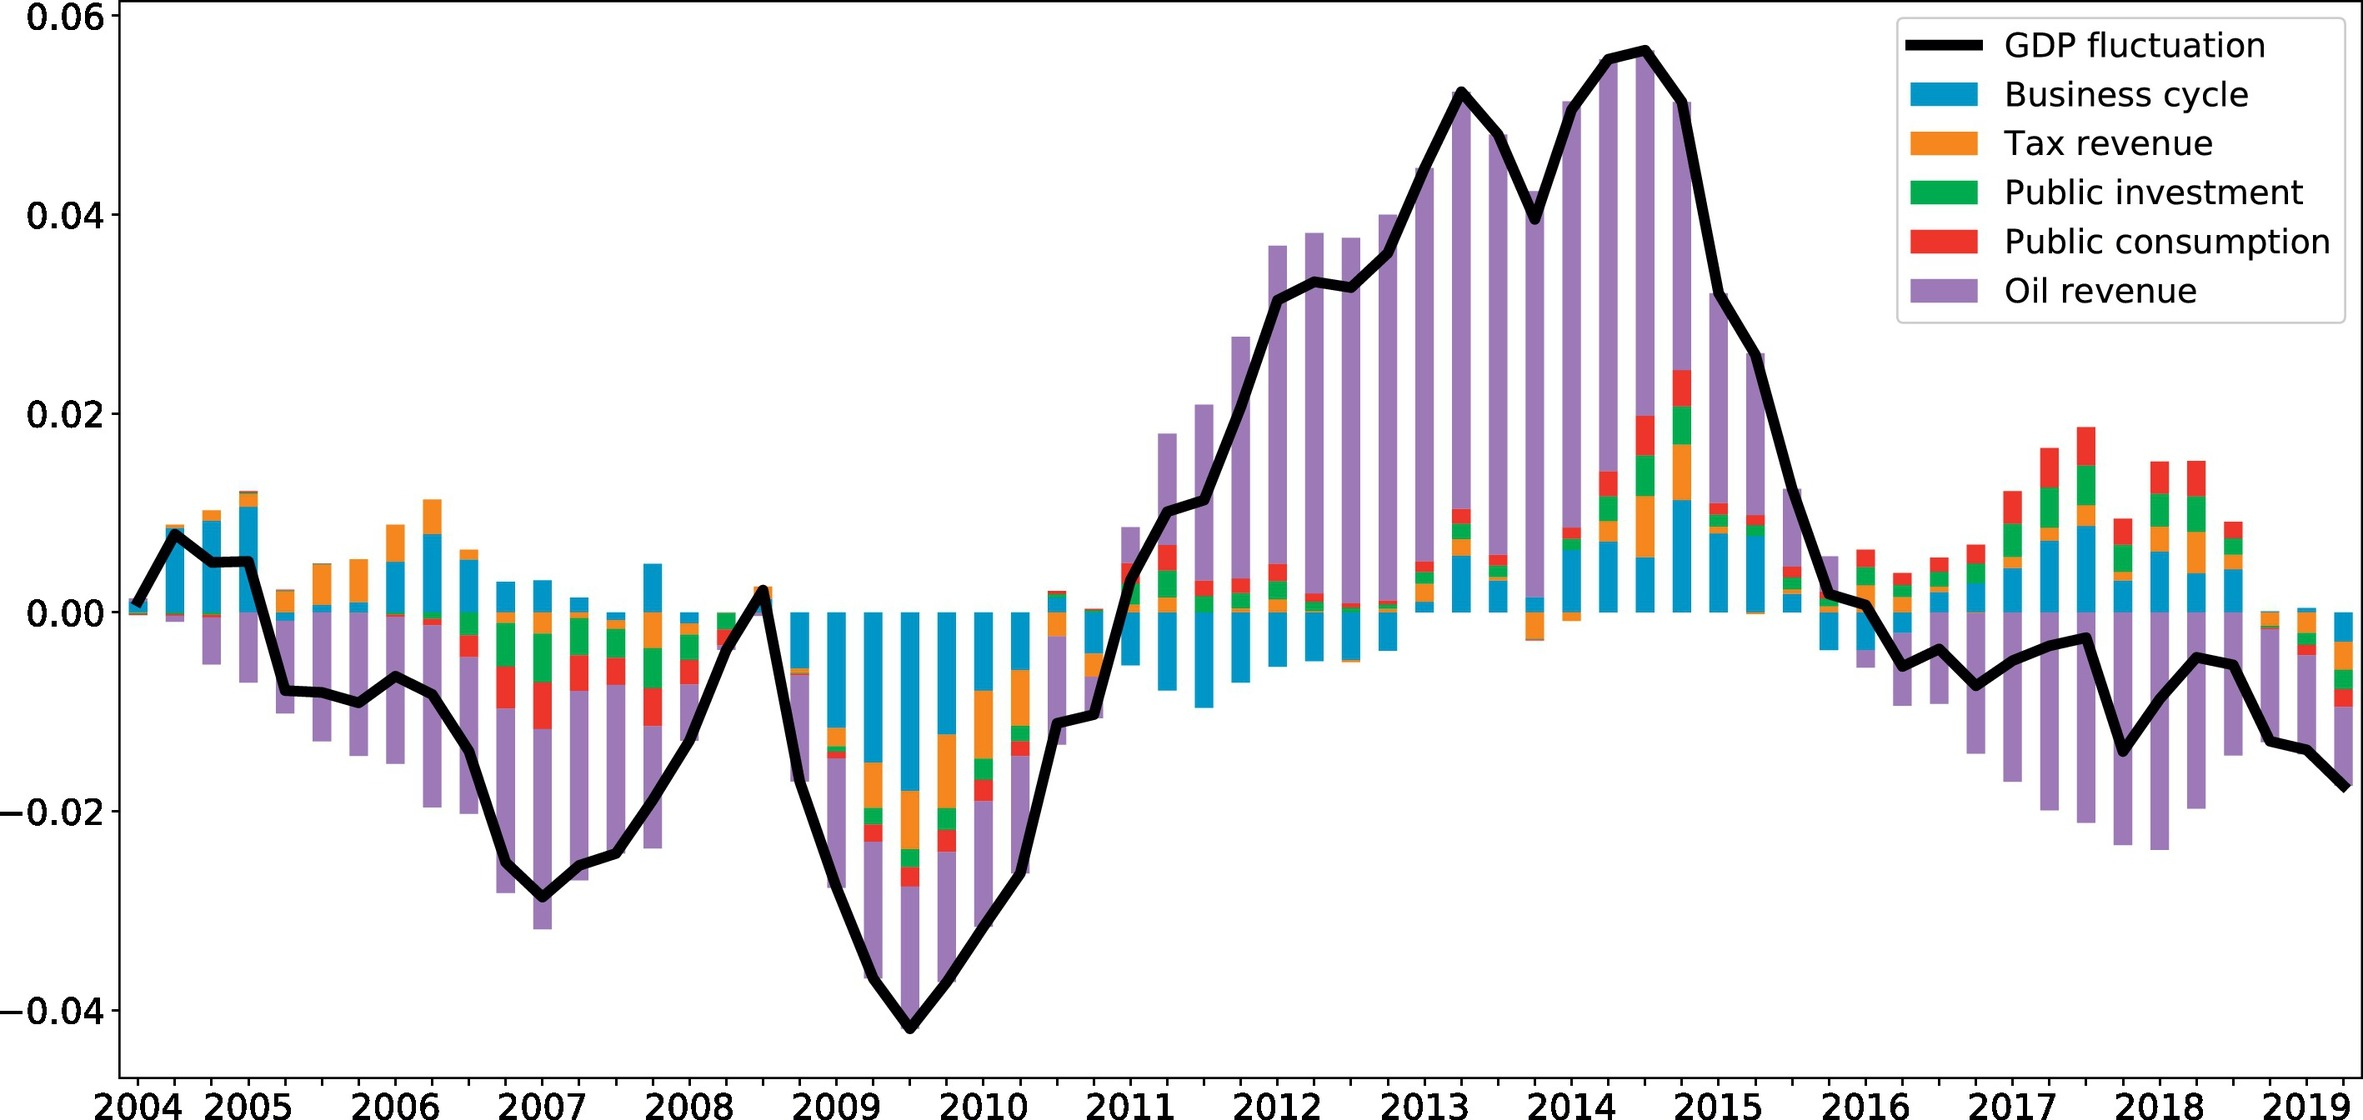
\includegraphics{images/Image1.png.jpg}
\caption{GDP fluctuations vs oil revenue between 2004-2019}
\end{figure}

\section{Motivation}\label{motivation}

\begin{itemize}
\item
  The oil well known as Block 43-ITT is located within Ecuador's Yasuní
  National Park---one of the most biodiverse places on Earth and home to
  Indigenous communities (UNESCO, 2024).
\item
  Oil exploitation in that well began in 2016 as part of efforts to
  boost fiscal revenues (Banco Central del Ecuador, 2023).
\item
  In the 2023 national referendum, the Ecuadorian population voted to
  halt extraction in that well (Corte Consitutional del Ecuador, 2023).
  \hspace{0pt}
\item
  The decision was driven by the growing environmental and Indigenous
  rights movement and marked a significant shift in Ecuador's natural
  resource policy.\hspace{0pt}
\end{itemize}

\section{Relevance}\label{relevance}

The government is now responsible for phasing out extraction while
addressing the economic implications---especially those related to oil
production levels and public revenues.\hspace{0pt}Evaluating how reduced
production affects overall output is critical for policy and planning
future decisions on resource management.

\section{Objective}\label{objective}

\begin{itemize}
\tightlist
\item
  This final project aims to forecast oil production in Ecuador for the
  forthcoming years, following the halt of extraction in Block 43-ITT,
  which raises questions about future national income.\hspace{0pt}
\end{itemize}

\begin{enumerate}
\def\labelenumi{\arabic{enumi}.}
\tightlist
\item
  \textbf{Quantitative Forecasting}~-- Produce monthly projections of
  national oil output through December~2027 under \emph{baseline} and
  \emph{halt} scenarios.
\item
  \textbf{Model Comparison}~-- Evaluate candidate models that
  accommodate seasonality, economic drivers, and structural breaks,
  selecting the most accurate and parsimonious specification.
\item
  \textbf{Decision Metrics}~-- Translate production deltas into fiscal
  terms (revenue and royalties), and present uncertainty ranges to guide
  policy trade‑offs.
\end{enumerate}

\section{Dataset information}\label{dataset-information}

\begin{itemize}
\tightlist
\item
  \textbf{Annual series:} Total barrels per year 1972--2024 (Government
  forecasts extend to 2029).
\item
  \textbf{Monthly series:} Jan~2007--Dec~2024 total production, WTI
  price, Block~43‑ITT output (2016--2023).
\end{itemize}

Data were cleaned and aligned in R; the annual series uses frequency~1,
monthly uses frequency~12. We focus annual analysis on 2000--2023 to
avoid pre‑2000 volatility.

\section{Analysis (Methods and
Models)}\label{analysis-methods-and-models}

\begin{itemize}
\item
  \textbf{Stage A} (Annual-Level Analysis):\hspace{0pt}

  \begin{itemize}
  \tightlist
  \item
    We use~an annual series (1972--2024) to analyze the long-run
    production trend.
  \end{itemize}
\item
  \textbf{Stage B} (Monthly-Level Analysis)\hspace{0pt}

  \begin{itemize}
  \item
    We use monthly dataset (2007--2024) for a more detailed
    (higher-frequency) forecast.\hspace{0pt}
  \item
    Additional variables:\hspace{0pt}

    \begin{itemize}
    \item
      Monthly WTI prices\hspace{0pt}
    \item
      Monthly block-level production of Block 43 ITT.
    \end{itemize}
  \end{itemize}
\item
  \textbf{Stage C} (Scenario analysis)\hspace{0pt}

  The idea~is that if we trust the long-run historical trend from the
  annual model, we can ensure that the sum our monthly forecasts matches
  the trend predicted by the annual model. \hspace{0pt}

  \begin{itemize}
  \item
    \textbf{Baseline forecast:} assuming Block 43 ITT continues as
    historical.\hspace{0pt}
  \item
    \textbf{Shutdown Scenario:} set Block 43 ITT output to zero in
    2024.\hspace{0pt}
  \end{itemize}
\end{itemize}

The difference in total production between the baseline and shutdown
forecasts is the gap that other blocks must fill to maintain the same
output level.\hspace{0pt}

\subsection{Stage A (Annual-Level
Analysis):}\label{stage-a-annual-level-analysis}

We used an annual series (1972--2024) to analyze the long-run production
trend.\hspace{0pt}

\subsubsection{Annual Data}\label{annual-data}

The chart below illustrates the trajectory of Ecuador's annual oil
output, which surged dramatically from the 1970s through the early
2000s. Following this period of rapid growth, production plateaued but
remained substantially higher than pre-2000 levels. By the early 2020s,
output had gradually declined to around 170 million barrels, possibly
influenced by aging fields, constrained investment, the effects of the
pandemic, or a combination of all.

The solely visualization may suggest that including data from before
2000 ---when output was only a fraction of its subsequent levels---
could distort our model's parameters. In contrast, restricting the
sample to the period from 2000 onward, when production stabilized at its
modern scale, is likely to yield a more accurate and relevant time
series and forecasts. Considering this, analyzing the Autocorrelation
Function (ACF) and Partial Autocorrelation Function (PACF) could provide
valuable insights for determining the most appropriate research period,
helping to identify patterns and lags in the data.

\includegraphics{FinalReport_V7_files/figure-latex/TSAnnual-1.pdf}

The sample ACF for the full series reveals strong autocorrelation
extending up to approximately the 15 lag, beyond which the correlations
sharply diminish, falling within the significance bounds for several
years. This decline signals that the pre-2000 data may not exhibit
meaningful memory. Similarly, the PACF presents a single significant
spike at lag 1, which may suggest an AR(1) structure for the series.

From that information and given that pre-2000 output levels are an order
of magnitude lower than post-2000 production and introduce disruptive
long-lag noise, we confined our model to the 2000--2023 period, aiming
at the model to gain precision and isolating the data's most relevant
structural characteristics.

\includegraphics{FinalReport_V7_files/figure-latex/plotACFPACF-1.pdf}

All the annual forecasting models were trained using data up to the year
2020. Because when using the pre-pandemic period, forecast performed
poorly (see Annex).

\subsubsection{Model 1: ARIMA}\label{model-1-arima}

The ``auto.arima'' in the training time series, suggests using the
ARIMA(0,1,0) model captures the general trend of Ecuador's oil
production over time but demonstrates moderate accuracy when handling
the data's inherent volatility (See Table 1). With a mean absolute
percent error (MAPE) of 0.94 (94\% error) and RMSE of approximately 2
million units, the model's performance is acceptable but not
exceptional. The forecast shows relatively stable future production
levels, though the wide confidence intervals (gray bands) indicate
substantial uncertainty in these predictions. The Theil's U value of
0.54 suggests that while the model outperforms naive forecasting
approaches, there remains considerable room for improvement in capturing
the time series' complex patterns and fluctuations.

\begin{verbatim}
##      Point Forecast     Lo 80     Hi 80     Lo 95     Hi 95
## 2021      175449722 161191369 189708074 153643453 197255990
## 2022      175449722 155285366 195614077 144611001 206288442
## 2023      175449722 150753530 200145913 137680157 213219286
\end{verbatim}

\includegraphics{FinalReport_V7_files/figure-latex/ARIMA-1.pdf}
\includegraphics{FinalReport_V7_files/figure-latex/ARIMA-2.pdf}

\subsubsection{Testing Model 2: MEAN}\label{testing-model-2-mean}

The Mean model employs a much simpler approach than ARIMA, that
generates a flat forecast (blue dots) at approximately 181 million
barrels with a wide confidence intervals, indicating high uncertainty.
Besides, its performance metrics (see Table 1) reveal significant
weaknesses, with a much higher RMSE (7,781,977) compared to ARIMA and a
concerning MAPE of 4.42 (442\% error). Moreover, according to the
model's Theil's U value of 2.77 indicates it performs worse than naive
forecasting methods, essentially failing to capture any of the time
series' patterns or fluctuations.

\begin{verbatim}
##      Point Forecast     Lo 80     Hi 80     Lo 95     Hi 95
## 2021      181558473 156628140 206488806 142320439 220796506
## 2022      181558473 156628140 206488806 142320439 220796506
## 2023      181558473 156628140 206488806 142320439 220796506
\end{verbatim}

\includegraphics{FinalReport_V7_files/figure-latex/MEAN-1.pdf}
\includegraphics{FinalReport_V7_files/figure-latex/MEAN-2.pdf}

\subsubsection{Testing Model 3: ETS}\label{testing-model-3-ets}

The ETS model effectively ``locks in'' the most recent observed level
(approximately 175 million barrels) and extrapolates it forward,
producing a flat forecast line characterized by moderately narrow
confidence bands. This tighter band of uncertainty, compared to the mean
model's wider fan, reflects ETS's ability to adapt to the stable, modern
production regime rather than being swayed by earlier, lower historical
levels.

In-sample (see Table 1), the model under-forecasts by an average of 1.6
million barrels (ME), achieving a MAPE below 1 percent (around 0.95\%).
A Theil's U statistic of 0.54 confirms that it outperforms a naive
``no-change'' forecast. However, the pronounced negative autocorrelation
at lag 1 indicates that the ETS model struggles to capture some of the
smoother, year-over-year momentum inherent in the data.

\begin{verbatim}
##      Point Forecast     Lo 80     Hi 80     Lo 95     Hi 95
## 2021      175451620 158940493 191962746 150200030 200703209
## 2022      175451620 152102567 198800672 139742325 211160914
## 2023      175451620 146855480 204047760 131717598 219185642
\end{verbatim}

\includegraphics{FinalReport_V7_files/figure-latex/ETS-1.pdf}
\includegraphics{FinalReport_V7_files/figure-latex/ETS-2.pdf}

\subsubsection{Testing Model 4: HOLT}\label{testing-model-4-holt}

Holt's method augments simple exponential smoothing with a linear trend,
and its forecast barely moves from the last observed level (around 175
million barrels), producing an almost flat‐looking line with even wider
uncertainty bands than ETS. It stands out that its Theil's U is 1.09,
which would suggests it actually performs worse than a naïve method.

\begin{verbatim}
##      Point Forecast     Lo 80     Hi 80     Lo 95     Hi 95
## 2021      176061114 159675163 192447065 151000965 201121263
## 2022      176670451 152596519 200744383 139852550 213488352
## 2023      177279788 146679865 207879711 130481244 224078332
\end{verbatim}

\includegraphics{FinalReport_V7_files/figure-latex/Holt-1.pdf}
\includegraphics{FinalReport_V7_files/figure-latex/Holt-2.pdf}

\subsubsection{Compare performance metrics of all models for the annual
analysis}\label{compare-performance-metrics-of-all-models-for-the-annual-analysis}

The following table compares the mentioned models accuracy, and shows
how ARIMA beats the rest of the models, while ETS is the second best
model

\begin{table}
\centering\centering
\caption{\label{tab:tablescores}Table 1. Forecast Accuracy for Annual Data}
\centering
\begin{tabular}[t]{l|r|r|r|r|r|r|r}
\hline
  & ME & RMSE & MAE & MPE & MAPE & ACF1 & Theil's U\\
\hline
\cellcolor{gray!10}{ARIMA} & \cellcolor{gray!10}{-1574422} & \cellcolor{gray!10}{2001707} & \cellcolor{gray!10}{1640694} & \cellcolor{gray!10}{-0.91057} & \cellcolor{gray!10}{0.94832} & \cellcolor{gray!10}{-0.61118} & \cellcolor{gray!10}{0.54238}\\
\hline
MEAN & -7683173 & 7781977 & 7683173 & -4.42404 & 4.42404 & -0.61118 & 2.77997\\
\hline
ETS & -1576320 & 2003200 & 1641327 & -0.91166 & 0.94870 & -0.61118 & 0.54288\\
\hline
HOLT & -2795151 & 3038681 & 2795151 & -1.61209 & 1.61209 & -0.65735 & 1.08959\\
\hline
\end{tabular}
\end{table}

\begin{verbatim}
## The best model by RMSE is: ARIMA
\end{verbatim}

\begin{verbatim}
## The best model by MAPE is: ARIMA
\end{verbatim}

Thus, we combined the two best models in aiming to have a more accurate
model. By feeding the ETS errors into a simple AR(1), this hybrid
forecast (red shading) sits almost exactly on today's production level
(around 175 million barrels) and produces the tightest uncertainty
``cone'' of all models. In back‐testing against 2021--2023 actuals (see
Table 2), it under‐forecasted by only 0.66 million barrels on average
(ME around --0.66 m), cutting its RMSE from \textasciitilde2.0 m (pure
ETS or ARIMA) down to 1.17 m and halving the MAPE to 0.54 \%. The
dramatic drop in MAE (to 0.93 m) and MAPE shows that capturing the
year-to-year autocorrelation in the residuals yields materially more
accurate point forecasts, while the narrower fan reflects increased
confidence in the short‐term outlook.

\begin{verbatim}
## [1] "ets_fc$lower.80%" "ets_fc$lower.95%"
\end{verbatim}

\begin{verbatim}
##   Year  Forecast      Lo80      Hi80      Lo95      Hi95
## 1 2021 173051133 140553653 205548612 123350527 222751738
## 2 2022 175137867 135666488 214609245 114771603 235504131
## 3 2023 175410611 130689832 220131390 107016082 243805140
\end{verbatim}

\includegraphics{FinalReport_V7_files/figure-latex/ETS.AR-1.pdf}

\begin{table}
\centering\centering
\caption{\label{tab:Accuracy2}Table 2. Forecast Accuracy for Annual Data}
\centering
\begin{tabular}[t]{l|r|r|r|r|r|r|r}
\hline
  & ME & RMSE & MAE & MPE & MAPE & ACF1 & Theil's U\\
\hline
ARIMA & -1574422.0 & 2001707 & 1640693.8 & -0.91057 & 0.94832 & -0.61118 & 0.54238\\
\hline
MEAN & -7683173.0 & 7781977 & 7683173.0 & -4.42404 & 4.42404 & -0.61118 & 2.77997\\
\hline
ETS & -1576320.2 & 2003200 & 1641326.5 & -0.91166 & 0.94870 & -0.61118 & 0.54288\\
\hline
HOLT & -2795151.5 & 3038681 & 2795151.5 & -1.61209 & 1.61209 & -0.65735 & 1.08959\\
\hline
\cellcolor{gray!10}{Hybrid ETS \& AR(1)} & \cellcolor{gray!10}{-657903.9} & \cellcolor{gray!10}{1171499} & \cellcolor{gray!10}{932078.9} & \cellcolor{gray!10}{-0.38062} & \cellcolor{gray!10}{0.53680} & \cellcolor{gray!10}{-0.40555} & \cellcolor{gray!10}{0.54320}\\
\hline
\end{tabular}
\end{table}

\begin{verbatim}
##                            ME    RMSE       MAE        MPE      MAPE       ACF1
## ARIMA              -1574422.0 2001707 1640693.8 -0.9105732 0.9483243 -0.6111825
## MEAN               -7683173.0 7781977 7683173.0 -4.4240445 4.4240445 -0.6111825
## ETS                -1576320.2 2003200 1641326.5 -0.9116649 0.9486952 -0.6111825
## HOLT               -2795151.5 3038681 2795151.5 -1.6120878 1.6120878 -0.6573494
## Hybrid ETS & AR(1)  -657903.9 1171499  932078.9 -0.3806204 0.5368018 -0.4055451
##                    Theil's U
## ARIMA              0.5423828
## MEAN               2.7799717
## ETS                0.5428761
## HOLT               1.0895856
## Hybrid ETS & AR(1) 0.5432020
\end{verbatim}

\begin{verbatim}
## The best model by RMSE is: Hybrid ETS & AR(1)
\end{verbatim}

\begin{verbatim}
## The best model by MAPE is: Hybrid ETS & AR(1)
\end{verbatim}

Now we use the hybrid model for our data from 2000 to 2023. This model
captured the long-term level and then added an AR(1) on its one-step
residuals to restore the small year-to-year momentum that pure ETS
missed. The outcome is a flat forecast of about 173 million barrels per
year from 2024 through 2027, with an 80 \% confidence band narrowing to
roughly 128--219 million and a 95 \% band of 103--244 million barrels.

\begin{verbatim}
## [1] "80%" "95%"
\end{verbatim}

\begin{verbatim}
## [1] "80%" "95%"
\end{verbatim}

\begin{verbatim}
##   Year  Forecast      Lo80      Hi80      Lo95      Hi95
## 1 2024 173209118 142864921 203553314 126801674 219616561
## 2 2025 173441171 136598394 210283947 117095006 229787335
## 3 2026 173470963 131733639 215208287 109639234 237302692
## 4 2027 173474788 127612784 219336792 103334906 243614670
\end{verbatim}

\includegraphics{FinalReport_V7_files/figure-latex/unnamed-chunk-1-1.pdf}

The residuals fluctuate randomly around zero with no obvious drift or
changing variance, and---aside from a single large error in the
mid-2000s---stay within about ±20 million barrels. Moreover, the ACF
shows all lags inside the 95 \% confidence bounds (lag 4 is barely
crossing the bounds, but we would say there is no meaningful serial
correlation). The histogram of errors looks symmetric (with slightly
tails from that outlier). In brief, they behave like white noise,
suggesting our hybrid ETS+AR(1) captured the main dynamics of Ecuador's
oil‐production series.

\includegraphics{FinalReport_V7_files/figure-latex/Residuals-1.pdf}

\begin{verbatim}
## 
##  Ljung-Box test
## 
## data:  Residuals from ETS(A,N,N)
## Q* = 8.0225, df = 5, p-value = 0.155
## 
## Model df: 0.   Total lags used: 5
\end{verbatim}

Finally, we observed that Ecuador's projected a higher production for
2026 \& 2027, however, there was no information on the additional data
they used for their forecasting. However it is worth noting that
projections for 2026 would be historic volumes as is slightly above
annual production in previous years.

\includegraphics{FinalReport_V7_files/figure-latex/unnamed-chunk-2-1.pdf}

\subsection{Stage B (Month-Level
Analysis):}\label{stage-b-month-level-analysis}

This is a more detailed monthly analysis from 2007--2023 using monthly
WTI prices and Block 43 production.

The following graphs shows oil production in Ecuador has been
decreasing. Oil extraction in Block 43-ITT started in 2016 and has
boosted the economy. Plot 4 shows that oil exploitation on Block 43-ITT
has increased production from 2016 to 2023, reaching up to 17\% of the
total oil production.

National production* shows clear 12‑month seasonality with shocks in
2020 (COVID‑19) and 2023 (maintenance outages). \emph{Block~43} exhibits
a steady upward trajectory until 2023; \emph{WTI} prices are markedly
cyclical with abrupt drops (2009,~2014,~2020).

\includegraphics{FinalReport_V7_files/figure-latex/1-1.pdf}

The left panel shows the ACF of the un‐differenced series. The
correlation at lag 0 is 1 and then decays only very gradually, remaining
significantly positive out to several seasonal cycles. Such a slow decay
is a signature of a non-stationary, trend-dominated process.
Superimposed on this decay are clear secondary peaks at lags ≈ 1.0, 2.0,
and 3.0 (i.e.~one-year, two-year, and three-year separations),
indicating a strong annual seasonal cycle in the data.

The right panel presents the PACF, which isolates the direct
(lag-by-lag) correlations after accounting for shorter lags. Here it is
showed a single dominant spike at lag 1, followed by very small (mostly
insignificant) bars---apart from pronounced seasonal spikes again at
whole-year lags. A rapid cutoff after lag 1 in the PACF is evidence
that, once the series is rendered stationary, an AR(1) term will capture
most of the short‐run dependence.

\textbf{Implications for Model Design}

\begin{itemize}
\item
  Non‐seasonal differencing (d = 1) is required to remove the
  slow-moving trend.
\item
  Seasonal differencing (D = 1 at lag s) is needed to eliminate the
  annual peaks in autocorrelation.
\item
  A single AR term (p = 1) suffices to model the remaining short‐lag
  dependence.
\item
  A seasonal AR or MA component at the annual lag (P or Q at lag s) will
  absorb any residual seasonal structure.
\end{itemize}

\includegraphics{FinalReport_V7_files/figure-latex/3-1.pdf}

The temporal split for models is as follows:

\begin{itemize}
\tightlist
\item
  \textbf{Training:} Jan~2007~--~Dec~2022 (192~obs).
\item
  \textbf{Validation:} Jan~2023~--~Dec~2023 (12~obs)~--- used solely for
  model selection.
\item
  \textbf{Test/Forecast:} Jan~2024~--~Dec~2027 (48~obs) under two
  scenarios.
\end{itemize}

\subsubsection{Model 1 - SARIMA}\label{model-1---sarima}

The ARIMA(0,1,2)(0,0,1){[}12{]} model successfully captures the overall
level and smooths regular seasonal swings in Ecuador's monthly oil
production, producing reasonable point forecasts and moderate
uncertainty bounds. However, remaining seasonal autocorrelation and
clustered shocks---evident in the residual ACF and Ljung--Box
test---indicate that the model fails to fully absorb annual patterns and
rare, large downturns.

\begin{verbatim}
##          Point Forecast    Lo 80    Hi 80    Lo 95    Hi 95
## Jan 2023       14928191 13486338 16370045 12723067 17133316
## Feb 2023       14556697 13045060 16068334 12244847 16868546
## Mar 2023       14785338 13262131 16308544 12455794 17114881
## Apr 2023       14717948 13183259 16252637 12370844 17065052
## May 2023       14774850 13228764 16320936 12410315 17139384
## Jun 2023       14395989 12838589 15953389 12014152 16777826
## Jul 2023       14740911 13172280 16309543 12341896 17139926
## Aug 2023       14791884 13212100 16371668 12375813 17207955
## Sep 2023       14718428 13127570 16309286 12285421 17151436
## Oct 2023       14788555 13186700 16390411 12338729 17238382
## Nov 2023       14714125 13101347 16326903 12247594 17180656
## Dec 2023       14901745 13278118 16525372 12418621 17384868
\end{verbatim}

\includegraphics{FinalReport_V7_files/figure-latex/model-sarima-1.pdf}
\includegraphics{FinalReport_V7_files/figure-latex/model-sarima-2.pdf}
\includegraphics{FinalReport_V7_files/figure-latex/model-sarima-3.pdf}

\begin{verbatim}
## 
##  Ljung-Box test
## 
## data:  Residuals from ARIMA(0,1,2)(0,0,1)[12]
## Q* = 48.566, df = 21, p-value = 0.0005756
## 
## Model df: 3.   Total lags used: 24
\end{verbatim}

\subsubsection{Model 2:}\label{model-2}

The StructTS basic structural model captures the smooth level and
seasonal shape of Ecuador's monthly oil production and yields stable,
well‐behaved forecasts. However, remaining seasonal autocorrelation and
the inability to fully accommodate sudden production drops---evidenced
by significant residual ACF spikes and a failed Ljung--Box
test---indicate the need for further refinement.

\begin{verbatim}
##          Point Forecast    Lo 80    Hi 80    Lo 95    Hi 95
## Jan 2023       15343823 13899091 16788556 13134296 17553351
## Feb 2023       14132564 12661291 15603838 11882446 16382683
## Mar 2023       15546772 14041285 17052258 13244328 17849215
## Apr 2023       14094481 12554828 15634135 11739785 16449178
## May 2023       14924654 13351495 16497813 12518715 17330593
## Jun 2023       14450412 12844335 16056490 11994129 16906696
## Jul 2023       15071488 13433006 16709971 12565646 17577331
## Aug 2023       15004106 13333748 16674464 12449514 17558699
## Sep 2023       14537057 12835545 16238570 11934818 17139296
## Oct 2023       14830601 13099271 16561932 12182760 17478443
## Nov 2023       14778439 13020417 16536462 12089776 17467103
## Dec 2023       14383272 12608586 16157957 11669124 17097419
\end{verbatim}

\includegraphics{FinalReport_V7_files/figure-latex/model-structts-1.pdf}
\includegraphics{FinalReport_V7_files/figure-latex/model-structts-2.pdf}
\includegraphics{FinalReport_V7_files/figure-latex/model-structts-3.pdf}

\begin{verbatim}
## 
##  Ljung-Box test
## 
## data:  Residuals from StructTS
## Q* = 58.197, df = 24, p-value = 0.0001143
## 
## Model df: 0.   Total lags used: 24
\end{verbatim}

\subsubsection{Model 3}\label{model-3}

TBATS excels at flexibly modeling complex seasonal patterns, producing
reasonable point forecasts and modestly narrow intervals. However, the
residual diagnostics reveal unmodeled seasonality (spike at lag 24).

\begin{verbatim}
##          Point Forecast    Lo 80    Hi 80    Lo 95    Hi 95
## Jan 2023       14810030 13517782 16102277 12833708 16786352
## Feb 2023       13972931 12595158 15350705 11865808 16080055
## Mar 2023       14970236 13573103 16367369 12833506 17106966
## Apr 2023       14012209 12600357 15424061 11852968 16171451
## May 2023       14248425 12822516 15674335 12067685 16429166
## Jun 2023       14606624 13167780 16045469 12406102 16807147
## Jul 2023       15129277 13678049 16580505 12909816 17348739
## Aug 2023       15256989 13793429 16720549 13018667 17495311
## Sep 2023       14197049 12722283 15671815 11941589 16452509
## Oct 2023       14860281 13373648 16346915 12586671 17133891
## Nov 2023       14256346 12759921 15752771 11967761 16544931
## Dec 2023       14821151 13313387 16328916 12515225 17127078
\end{verbatim}

\includegraphics{FinalReport_V7_files/figure-latex/model-tbats-1.pdf}
\includegraphics{FinalReport_V7_files/figure-latex/model-tbats-2.pdf}
\includegraphics{FinalReport_V7_files/figure-latex/model-tbats-3.pdf}

\begin{verbatim}
## 
##  Ljung-Box test
## 
## data:  Residuals from TBATS
## Q* = 63.515, df = 24, p-value = 2.005e-05
## 
## Model df: 0.   Total lags used: 24
\end{verbatim}

\subsubsection{Model 4}\label{model-4}

ETS model anchors all predictions to the final smoothed value. It
performs respectably as a baseline---its MAPE of 3.56 \% places it among
the top five models---but fails to capture both trend and seasonality,
as evidenced by seasonal autocorrelation and shock‐clustering in the
residuals.

\begin{verbatim}
##          Point Forecast    Lo 80    Hi 80    Lo 95    Hi 95
## Jan 2023       14661274 13194535 16128013 12418090 16904458
## Feb 2023       14661274 13177242 16145306 12391643 16930905
## Mar 2023       14661274 13160149 16162399 12365501 16957047
## Apr 2023       14661274 13143248 16179300 12339654 16982895
## May 2023       14661274 13126533 16196015 12314090 17008458
## Jun 2023       14661274 13109998 16212550 12288803 17033746
## Jul 2023       14661274 13093638 16228910 12263782 17058767
## Aug 2023       14661274 13077447 16245102 12239019 17083529
## Sep 2023       14661274 13061419 16261129 12214507 17108041
## Oct 2023       14661274 13045551 16276998 12190238 17132310
## Nov 2023       14661274 13029836 16292712 12166205 17156343
## Dec 2023       14661274 13014272 16308276 12142402 17180146
\end{verbatim}

\includegraphics{FinalReport_V7_files/figure-latex/model-ets-1.pdf}
\includegraphics{FinalReport_V7_files/figure-latex/model-ets-2.pdf}
\includegraphics{FinalReport_V7_files/figure-latex/model-ets-3.pdf}

\begin{verbatim}
## 
##  Ljung-Box test
## 
## data:  Residuals from ETS(A,N,N)
## Q* = 51.347, df = 24, p-value = 0.0009511
## 
## Model df: 0.   Total lags used: 24
\end{verbatim}

\subsubsection{Model 5}\label{model-5}

We regress deseasonalized monthly production on the WTI price only, then
model the residuals as an ARIMA(0,1,2)(2,0,0){[}12{]} process. This
specification delivers a hold‐out MAPE of 3.76 \%, making it our most
accurate well‐behaved model.The WTI regressor explains the bulk of level
shifts and low-frequency seasonal effects; the
ARIMA(0,1,2)(2,0,0){[}12{]} errors then capture residual
autocorrelation.

\begin{verbatim}
##          Point Forecast    Lo 80    Hi 80    Lo 95    Hi 95
## Jan 2023       15040482 13623432 16457533 12873291 17207674
## Feb 2023       14164622 12652105 15677139 11851427 16477817
## Mar 2023       14641464 13117464 16165464 12310707 16972221
## Apr 2023       14558761 13023363 16094158 12210573 16906949
## May 2023       14592767 13046056 16139478 12227276 16958258
## Jun 2023       13987292 12429349 15545234 11604624 16369959
## Jul 2023       14557435 12988341 16126529 12157714 16957157
## Aug 2023       14658232 13078066 16238398 12241577 17074887
## Sep 2023       14581468 12990307 16172629 12147997 17014939
## Oct 2023       14661034 13058953 16263115 12210863 17111206
## Nov 2023       14420684 12807757 16033611 11953925 16887442
## Dec 2023       13272391 11648691 14896091 10789156 15755626
\end{verbatim}

\includegraphics{FinalReport_V7_files/figure-latex/model-arimax-1.pdf}
\includegraphics{FinalReport_V7_files/figure-latex/model-arimax-2.pdf}
\includegraphics{FinalReport_V7_files/figure-latex/model-arimax-3.pdf}

\begin{verbatim}
## 
##  Ljung-Box test
## 
## data:  Residuals from Regression with ARIMA(0,1,2)(2,0,0)[12] errors
## Q* = 45.22, df = 20, p-value = 0.00103
## 
## Model df: 4.   Total lags used: 24
\end{verbatim}

\subsubsection{Compare performance metrics of all
models}\label{compare-performance-metrics-of-all-models}

\begin{verbatim}
##                  ME     RMSE      MAE         MPE     MAPE       ACF1 Theil's U
## SARIMA   -278293.15 693303.0 406561.4 -2.16415262 3.017604 0.17326075 0.7240965
## StructTS -301877.35 728247.7 447376.6 -2.29073820 3.261772 0.32730412 0.8107510
## TBATS    -138867.29 619140.1 477062.0 -1.14463527 3.434871 0.19380236 0.6598076
## ETS      -205012.18 738631.1 486261.3 -1.68608859 3.558863 0.03492328 0.7520508
## Arimax_p   28209.18 777434.1 526220.8 -0.04530021 3.758984 0.29258131 0.8122824
\end{verbatim}

\begin{verbatim}
## The best model by RMSE is: TBATS
\end{verbatim}

\includegraphics{FinalReport_V7_files/figure-latex/forecast-comparison-1.pdf}

\begin{table}
\centering\centering\centering
\caption{\label{tab:forecast-accuracy-kable}Forecast Accuracy for Monthly Data}
\centering
\begin{tabular}[t]{l|r|r|r|r|r|r|r}
\hline
  & ME & RMSE & MAE & MPE & MAPE & ACF1 & Theil's U\\
\hline
SARIMA & -278293.15 & 693303.0 & 406561.4 & -2.16415 & 3.01760 & 0.17326 & 0.72410\\
\hline
StructTS & -301877.35 & 728247.7 & 447376.6 & -2.29074 & 3.26177 & 0.32730 & 0.81075\\
\hline
\cellcolor{gray!10}{TBATS} & \cellcolor{gray!10}{-138867.29} & \cellcolor{gray!10}{619140.1} & \cellcolor{gray!10}{477062.0} & \cellcolor{gray!10}{-1.14464} & \cellcolor{gray!10}{3.43487} & \cellcolor{gray!10}{0.19380} & \cellcolor{gray!10}{0.65981}\\
\hline
ETS & -205012.18 & 738631.1 & 486261.3 & -1.68609 & 3.55886 & 0.03492 & 0.75205\\
\hline
\cellcolor[HTML]{F0F0F0}{\textbf{Arimax\_p}} & \cellcolor[HTML]{F0F0F0}{\textbf{28209.18}} & \cellcolor[HTML]{F0F0F0}{\textbf{777434.1}} & \cellcolor[HTML]{F0F0F0}{\textbf{526220.8}} & \cellcolor[HTML]{F0F0F0}{\textbf{-0.04530}} & \cellcolor[HTML]{F0F0F0}{\textbf{3.75898}} & \cellcolor[HTML]{F0F0F0}{\textbf{0.29258}} & \cellcolor[HTML]{F0F0F0}{\textbf{0.81228}}\\
\hline
\end{tabular}
\end{table}

The only model among these whose residuals truly behave like white noise
is the \textbf{regression-with-ARIMA-errors} approach using the WTI-only
regressor (Arimaxₚ). Its slightly higher MAPE is more than offset by the
diagnostic clearance---making it the \textbf{best overall choice} for
reliable forecasting and counterfactual scenario analysis.

\section{Scenario Analysis}\label{scenario-analysis}

After identifying the price-only ARIMAX (with
ARIMA(0,1,2)(2,0,0){[}12{]} errors) as our preferred monthly forecasting
engine, we simulated two contrasting futures for January 2024--December
2025:

\begin{itemize}
\item
  Baseline -- all blocks, including Block 43-ITT, continue producing at
  their most recently observed levels (with WTI prices at their
  2019--2023 average).
\item
  Shutdown -- Block 43-ITT production is set to zero from September 2024
  onward; everything else follows the same inputs.
\end{itemize}

\begin{verbatim}
##          Point Forecast    Lo 80    Hi 80    Lo 95    Hi 95
## Jan 2023       15040482 13623432 16457533 12873291 17207674
## Feb 2023       14164622 12652105 15677139 11851427 16477817
## Mar 2023       14641464 13117464 16165464 12310707 16972221
## Apr 2023       14558761 13023363 16094158 12210573 16906949
## May 2023       14592767 13046056 16139478 12227276 16958258
## Jun 2023       13987292 12429349 15545234 11604624 16369959
## Jul 2023       14557435 12988341 16126529 12157714 16957157
## Aug 2023       14658232 13078066 16238398 12241577 17074887
## Sep 2023       14581468 12990307 16172629 12147997 17014939
## Oct 2023       14661034 13058953 16263115 12210863 17111206
## Nov 2023       14420684 12807757 16033611 11953925 16887442
## Dec 2023       13272391 11648691 14896091 10789156 15755626
\end{verbatim}

From September 2024 onward, the shutdown path lies uniformly below the
baseline---by exactly the block-43 contribution we estimated (≈ 1 656
682 barrels/month).

\begin{itemize}
\item
  \textbf{Average monthly shortfall:} 1.66 million barrels
\item
  \textbf{Total 2-year loss:} 19.88 million barrels
\end{itemize}

This gap represents the additional output that must be found in oil
blocks if national production is to remain on the baseline trajectory.

\begin{verbatim}
## Production gap (per month):
\end{verbatim}

\begin{verbatim}
##          Jan     Feb     Mar     Apr     May     Jun     Jul     Aug     Sep
## 2023 1656682 1656682 1656682 1656682 1656682 1656682 1656682 1656682 1656682
##          Oct     Nov     Dec
## 2023 1656682 1656682 1656682
\end{verbatim}

\begin{verbatim}
## Average monthly production gap: 1656682
\end{verbatim}

\begin{verbatim}
## Total production gap over the forecast period: 19880180
\end{verbatim}

\includegraphics{FinalReport_V7_files/figure-latex/scenario-plot-1.pdf}

\begin{verbatim}
## Time Series:
## Start = 2023 
## End = 2038 
## Frequency = 1 
##  [1] 172376758 175661395 170261829 172609726 174764658 174617716 175128024
##  [8] 174466453 168261695 167487461 168561507 170514383 169415364 166948600
## [15] 170946978 174636167
\end{verbatim}

By summing our monthly forecasts into annual totals, we compare:

\begin{itemize}
\item
  Historical annual production (2000--2023) in blue
\item
  Aggregated baseline forecast (2024--2038) in red
\item
  Aggregated shutdown forecast (not shown but would track the baseline
  minus ≈ 19.9 million in 2025)
\end{itemize}

\textbf{Without Block 43}, Ecuador's total oil output falls from
\textbf{≈ 172 million barrels} (baseline) to \textbf{≈ 152 million
barrels}, a \textbf{12 \% drop}.

\includegraphics{FinalReport_V7_files/figure-latex/annual-forecast-plot-1.pdf}

\section{Summary and Conclusions}\label{summary-and-conclusions}

Halting Block~43‑ITT aligns with conservation aims but carries a
material macro‑fiscal cots. Strategic technical and financial measures
can limit losses to \textasciitilde7~\% of national output by 2027;
without them, Ecuador faces a pronounced revenue shock in 2025.

\section*{References}\label{references}
\addcontentsline{toc}{section}{References}

\phantomsection\label{refs}
\begin{CSLReferences}{1}{0}
\bibitem[\citeproctext]{ref-banco_central_del_ecuador_estudio_2023}
Banco Central del Ecuador. (2023). Estudio de los impactos
macroeconómicos de mantener el crudo del Bloque 43-ITT indefinidamente
en el subsuelo. \emph{74}.
\url{https://contenido.bce.fin.ec/documentos/PublicacionesNotas/Catalogo/Apuntes/ae74.pdf}

\bibitem[\citeproctext]{ref-corteconsitutionaldelecuadorCaseNo622CP2023}
Corte Consitutional del Ecuador. (2023). \emph{Case no. 6-22-CP}.
\url{http://esacc.corteconstitucional.gob.ec/storage/api/v1/10_DWL_FL/e2NhcnBldGE6J3RyYW1pdGUnLHV1aWQ6JzYwMjJlYzc1LWViYzctNDNjYi05MjJjLWUyOTVhN2I4OTBjMy5wZGYnfQ==}

\bibitem[\citeproctext]{ref-unescoMainInitiativesYasuni2024}
UNESCO. (2024). \emph{Main initiatives in the {Yasun{í} Biosphere
Reserve}, {Ecuador} {\textbar} {UNESCO}}.
https://www.unesco.org/en/amazon-biosphere-reserves-project/yasuni.

\end{CSLReferences}

\end{document}
